\documentclass[a4paper,11pt]{article}

\usepackage[svgnames]{xcolor}
\usepackage{a4wide}
\usepackage{tikz}
\usetikzlibrary{arrows,pgfplots.groupplots}
\usepackage{pgfplots}
\pgfplotsset{compat=1.3}
\usepackage[detect-family]{siunitx}
\usepackage[eulergreek]{sansmath}
\sisetup{text-sf=\sansmath}
\usepackage{relsize}

\pagestyle{empty}

\begin{document}
% !TeX root = thesis.tex
% Based on station-layout.tex from Fokkema 2013.

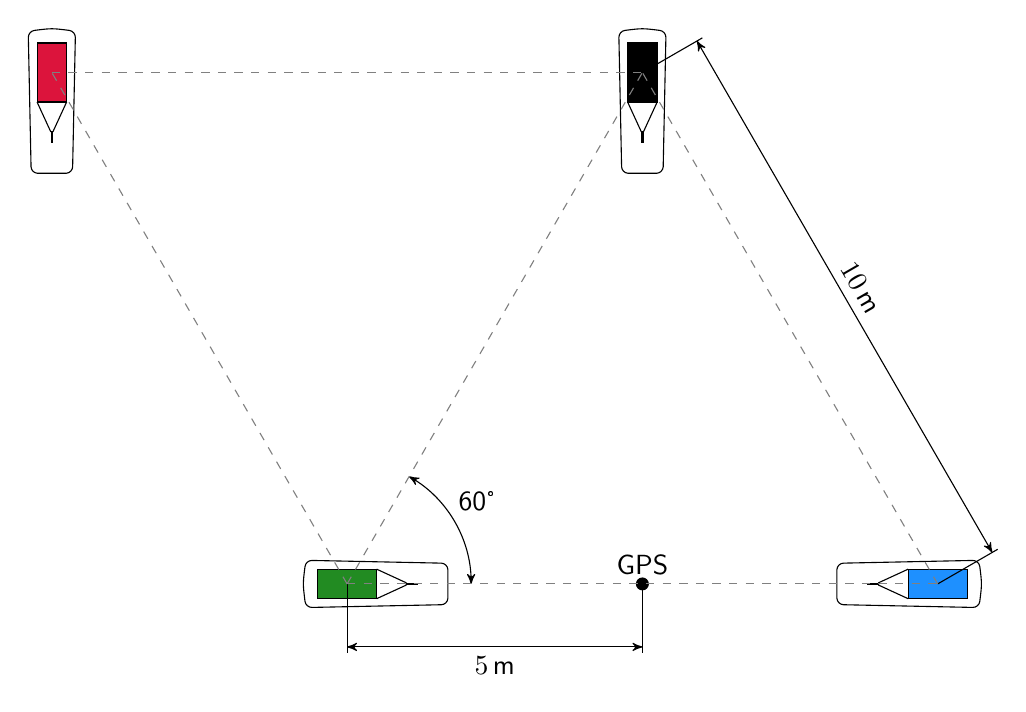
\begin{tikzpicture}
    [ font=\sffamily, x=.75cm, y=.75cm,
      hisparc/.style={draw},
      >=stealth',
    ]
    \foreach \col / \sx / \sy / \angle in {ForestGreen/-5/0/90, DodgerBlue/5/0/-90,
                                           Crimson/-10/8.66/0, black/0/8.66/0} {
        \begin{scope}[hisparc, shift={(\sx,\sy)}, rotate=\angle]
            \draw[rounded corners=2.25pt]
                (-.4, .7) .. controls (0, .75) ..  (.4, .7) -- 
                (.35, -1.7) ..  controls(0, -1.72) ..  (-.35, -1.7) --
                cycle;
            \draw[fill=\col] (-.25, .5) rectangle (.25, -.5);
            \draw (-.25, -.5) -- (-.02, -1) --(.02, -1) -- (.25, -.5);
            \fill (-.02, -1) rectangle (.02, -1.2);
        \end{scope}
    }
    \draw[fill] (0, 0) circle (.10) node [above] {GPS};
%    \node[color=gray] at (-5, .75) {\Large 0};
%    \node[color=gray] at (5, .75) {\Large 1};
%    \node[color=gray] at (-.75, 8.1) {\Large 2};
%    \node[color=gray] at (-9.25, 8.1) {\Large 3};

    \coordinate (A) at (-5, 0);
    \coordinate (B) at (5, 0);
    \coordinate (D) at (0, 8.66);
    \coordinate (F) at (-10, 8.66);

    \coordinate (A') at ($ (A)!.8cm!-90:(B) $);
    \coordinate (B') at ($ (B)!.8cm!90:(A) $);
%    \draw (A) -- ($ (A)!1.1!(A') $);
%    \draw (B) -- ($ (B)!1.1!(B') $);
%    \draw[<->] (A') -- (B') node [midway, below] {\SI{10}{\meter}};

    \coordinate (C') at ($ (B)!.8cm!-90:(D) $);
    \coordinate (D') at ($ (D)!.8cm!90:(B) $);
    \draw (B) -- ($ (B)!1.1!(C') $);
    \draw (D) -- ($ (D)!1.1!(D') $);
    \draw[<->] (C') -- (D') node [midway, above, sloped] {\SI{10}{\meter}};

    \coordinate (E) at (0, 0);
    \coordinate (D'') at ($ (D)!.8cm!180:(E) $);
    \coordinate (E') at ($ (E)!.8cm!90:(A) $);
    \coordinate (F') at ($ (F)!.8cm!-90:(D) $);
%    \draw (F) -- ($ (F)!1.1!(F') $);
%    \draw (D) -- ($ (D)!1.1!(D'') $);
%    \draw[<->] (F') -- (D'') node [midway, below, sloped] {\SI{10}{\meter}};
    \draw (A) -- ($ (A)!1.1!(A') $);
    \draw (E) -- ($ (E)!1.1!(E') $);
    \draw[<->] (A') -- (E') node [midway, below] {\SI{5}{\meter}};

    \draw[<->] (A) ++(0:2.1) arc (0:60:2.1);
    \node at (-2.8, 1.4) {60°};

    \draw[dashed,gray] (A) -- (B);
    \draw[dashed,gray] (A) -- (D);
    \draw[dashed,gray] (B) -- (D);
    \draw[dashed,gray] (A) -- (F);
    \draw[dashed,gray] (F) -- (D);
%    \draw[dashed,gray] (A) -- (F);
\end{tikzpicture}

\end{document}
